 % * 
% * picoFlamingo: 3D Portable Presentation System
% * Copyright (c) 2010, 2011 David Mart�nez Oliveira
% *
% * This file is part of picoFlamingo
% *
% * picoFlamingo is free software: you can redistribute it and/or modify
% * it under the terms of the GNU General Public License as published by
% * the Free Software Foundation, either version 3 of the License, or
% * (at your option) any later version.
% *
% * picoFlamingo is distributed in the hope that it will be useful,
% * but WITHOUT ANY WARRANTY; without even the implied warranty of
% * MERCHANTABILITY or FITNESS FOR A PARTICULAR PURPOSE.  See the
% * GNU General Public License for more details.
% *
% * You should have received a copy of the GNU General Public License
% * along with picoFlamingo.  If not, see <http://www.gnu.org/licenses/>.
% *

\documentclass[10pt,a4paper,twoside]{article}

\usepackage[latin1]{inputenc}                                 
\usepackage[english]{babel} 

\usepackage{graphicx}
\usepackage{a4,fancyhdr, multicol}
\usepackage{float}
\usepackage{pdftricks}
\usepackage{pstricks}
\usepackage{color}
\usepackage{pst-plot}
\usepackage{pst-eps}
\usepackage{wrapfig}
\usepackage{eso-pic}
\usepackage{listings}
\usepackage{textpos}
\usepackage{epsf}
\usepackage{setspace}
\usepackage{hyperref}
\usepackage{colortbl}


\setlength{\parindent}{0.0in}

\setlength{\oddsidemargin}{0.05mm}
\setlength{\evensidemargin}{0.05mm}

\addtolength{\textwidth}{2cm}
\addtolength{\topmargin}{-1.5cm}


\setlength{\parskip}{0.1cm}

\newcommand{\EOP}{\psframe[fillstyle=solid, fillcolor=darkred,linecolor=darkred](-20,0.4)(20cm, -1.0cm)}


\pagestyle{fancy}

\fancyfoot[CO,CE]{}
\fancyhead[RO,LE]{{\color{darkred}{\textbf{\textsf{Last Updated\\ \today}}}}}
\fancyhead[LO,RE]{{\color{darkred}{\textbf{\textsf{{\textbf{\textsf{picoFlamingo\\PROJECT}}}}}}}}


\fancyfoot[LE]{\EOP{\color{white}{\textbf{\textsf{The Cracking EGG |
          User Manual}}}}}
\fancyfoot[RO]{{\color{white}{\textbf{\textsf{The Cracking EGG |
          UserManual}}}}}

\fancyfoot[LO]{\EOP{\color{white}{\textbf{\textsf{\thepage}}}}}
\fancyfoot[RE]{{\color{white}{\textbf{\textsf{\thepage}}}}}


\renewcommand{\footrulewidth}{0.0pt}
\renewcommand{\headrulewidth}{0.4pt}


\definecolor{darkred}{rgb}{0.4,0.1,0.1}

% Configuraci�n de Hyperenlaces.
% Uso del paquete hyperref sugerido por Cruz Enrique Borges Hern�ndez
\hypersetup{
    bookmarks=true,        % show bookmarks bar?
    colorlinks=true,       % false: boxed links; true: colored links
    linkcolor=darkred,         % color of internal links
    citecolor=green,       % color of links to bibliography
    filecolor=magenta,     % color of file links
    urlcolor=darkred          % color of external links
}



\makeindex

\begin{document}

% Portada
%%%%%%%%%%%%%%%%%%%%%%%%%%%%%%%%%%%%%%%%%%%%%%%%%%%

\pagestyle{empty}

% Put Images
\rput(8,-1.0){\resizebox{!}{10cm}{{\epsfbox{images/front_pag_header.eps}}}}
\rput(13,-16.0){\resizebox{!}{10cm}{{\epsfbox{images/front_page_logo1.eps}}}}



\vspace{1mm}


\vspace{2mm}



\begin{textblock}{30}(1.5, -0.5)
{\color{white}{{\resizebox{15cm}{0.6cm}{{\textsf{picoFlamingo Alpha
            0.4. User Manual}}}}}}
\medskip

{\color{white}{{\resizebox{7cm}{!}{{{\textsf{Codename: {\textbf{``The Cracking Egg''}}}}}}}}}
\end{textblock}


\begin{textblock}{30}(1.5, 1.2)
{\color{darkred}{{\resizebox{7cm}{0.3cm}{{\textsf{Edition 0 Rev 1 DRAFT by DMO}}}}}}

{\color{darkred}{{\large{\textsf{\today}}}}}
\end{textblock}



\begin{textblock}{30}(-1.5, 13)


{{\color{darkred}{{\textsf{\textbf{picoflamingo@papermint-designs.com}}}}}}

{{\color{darkred}{\textsf{\textbf{{http://www.papermint-designs.com/picoflamingo}}}}}}

{{\color{darkred}{\textsf{\textbf{{http://www.papermint-designs.com/community/?q=blog/3}}}}}}

\end{textblock}

\rput(20.0, -23.5)
{\psset{linecolor=darkred}\psline(-30,0)}

\clearpage
\pagebreak

\vspace{2cm}

(c) Papermint Designs,  2009, 2011

\vspace{5mm}

This document is distributed under a Creative Commons License SA-BY.


This work is licenced under the Creative Commons Attribution-Share
Alike 3.0 Unported License. To view a copy of this licence, visit
{\url{http://creativecommons.org/licenses/by-sa/3.0/}} or send a letter to
Creative Commons, 171 Second Street, Suite 300, San Francisco,
California 94105, USA.


\clearpage
\pagebreak

\pagestyle{fancy}

.

\pagebreak



\tableofcontents

\clearpage
\pagebreak



%%%%%%%%%%%%%%%%%%%%%%%%%%%%%%%%%%%%%%%%%%%%%%%%%%%%%%%%%%%%%%%%%
%%%%%%%%%%%%%%%%%%%%%%%%%%%%%%%%%%%%%%%%%%%%%%%%%%%%%%%%%%%%%%%%%
%%%%%%%%%%%%%%%%%%%%%%%%%%%%%%%%%%%%%%%%%%%%%%%%%%%%%%%%%%%%%%%%%

\clearpage
\pagebreak
\section{Introduction}

picoFlamingo is a lightweight presentation system intended to be
deployed on embedded systems and therefore be really portable. The
currently chosen hardware platform for the development is the
BeagleBoard (\url{http://beagleboard.org}), as processing unit, and the
Texas Instruments {\href{http://focus.ti.com/dlpdmd/docs/dlpdiscovery.tsp?sectionId=60&tabId=2235}{picoDLP}} projector.

The small power fingerprint and size of booth system makes
them a very good tandem for the picoFlamingo project.

The intended audience of the system are professional that need to
present their works in an attractive way to small audiences, anywhere
at any time. Specially the ones that need 3D capabilities to show, for instance,
their product concepts (no physically available) or products too huge for a meeting room.

This document covers the release of the second alpha version of
the system (code name ``The Cracking Egg''), including system installation,
configuration and operation.

\subsection{Features of this Release}

The features of picoFlaming alpha 0.4, ``The Cracking Egg'', release are:

\begin{itemize}
\item The following slide items are allowed:
\begin{itemize}
\item Text. Several different True-Type fonts can be used to add text to the slides.
\item Image. Several different image formats can be used to add images
  to the slide
\item 3D Models in 3DS file format.
\item Live video streams
\end{itemize}

\item All item in slide are visualised in a 3D space. Position and
  Orientation can be changed for any item

\item In Slide animation of any item

\item Predefined slides transitions

\item Slide show mode

\item Different Remote Control options

\item OpenGL ES 2.0. Frame buffer and X11 versions.

\begin{itemize}

\item Remote control through Bluetooth or TCP/IP (wired or wifi
  depending on configured hardware). 
\item Simple remote control application for Symbian Devices using
  Python S60, allowing the navigation throughout the presentation
\item Simple remote control application for FreeRunner OpenMoko and
  Linux boxes with X11/SDL graphics and Bluetooth or Networking
  capabilities. This application allows rotation of the selected item
  in the presentation.
\item Simple Android remote control version. Not included in distribution.
\end{itemize}

\item Additional tools and utilities

\begin{itemize}
\item Simple Voice commanding solution for navigating presentations
\item Simple Video streamer for v4l2 devices
\item Basic button agent for building simple interfaces
\end{itemize}


\end{itemize}


\begin{figure}[ht]
\centering
  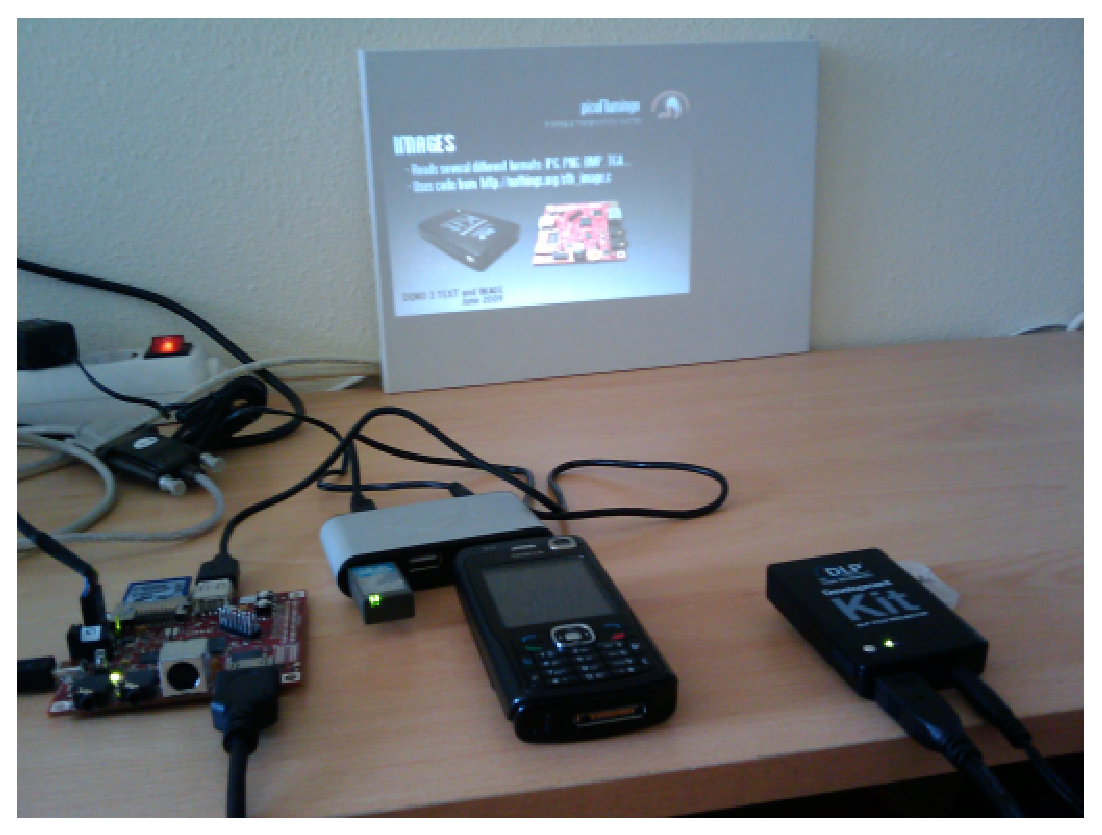
\includegraphics[width=1.0\hsize,angle=0]{images/pink-egg-hw.eps}
{\small{\caption{\label{fig:pink-egg-hw}The ``Cracking Egg'' system at
  Papermint Designs Lab}}}
\end{figure}



\clearpage
\pagebreak


\section{System Overview}

This section describes the hardware and software environment required
by the system as well as the installation process for the ``The Cracking
Egg'' different components.

\subsection{Software Components}

The picoFlamingo ``Cracking Egg'' is composed of the following minimal
software components:

\begin{itemize}

\item {\textbf{The NetKitty communications tool}}. This is an small program that
  allows Bluetooth and TCP connectivity. The picoFlamingo application
  uses it and the redirection of the standard input to get remote
  commands. The extended remote control application, uses it and the
  redirection of standard output to send control messages to the presentation.


\item {\textbf{The picoFlamingo application}}. This is the main application in
  charge of controlling the presentation. The picoFlamingo application
  renders the slides and exposes remote commands to control the
  navigation through the presentation.

  This application needs the Netkitty communication tool for remote operation.

\item {\textbf{The simplified remote control application for Python S60}}. This
  is a simple python script that can be executed in Symbian S60
  devices and uses the Bluetooth interface for navigating a
  picoFlamingo ``Cracking Egg'' presentation remotely. This application
  only supports moving to the next and previous slide.

\item {\textbf{The extended remote control application for OpenMoko FR and
  Linux Boxes}}. This is an SDL application providing extended
  functionalities for remote controlling the picoFlamingo ``Cracking
  Egg''. In addition to forward and backward slide navigation, this
  application allows to rotate a given object (this is defined in the
  presentation itself) within the presentation in real-time.

  This application needs the Netkitty communication tool for remote operation.
\end{itemize}

\subsection{Tested Hardware}

The ``Cracking Egg'' has been tested using the following hardware:

\begin{itemize}

\item The picoFlamingo ``Cracking Egg'' has been tested on the
  following hardware
\begin{itemize}
\item BeagleBoard Revisions B6 and C3. 

\item x86 PC compatible computers. 

\item Omap Zoom II

\item OMAP4 Blaze

\end{itemize}

\item The extended Remote Control application has been tested on the
  following hardware
\begin{itemize}
\item x86 PC compatible computers. 

\item Omap Zoom II

\item OpenMoko FreeRunner
\end{itemize}


\item Nokia N70 Symbian device

Runs the simplified remote control application for Python S60.


\item picoDLP projector

Used for portable projection of the presentation from the BeagleBoard.

\item USB Bluetooth dongle.

Used for remote wireless Bluetooth connectivity.

\end{itemize}

As an alpha release no extensive testing has been done, however the
system should work with other configurations without major problems.

\subsection{Software Requirements}
\label{sw-deps}
The ``Cracking Egg'' needs the following additional software components to run.

\begin{itemize}
\item OpenGL ES 2.0 support. The OpenGL ES 2.0 user libraries (and
  hardware drivers) for the Beagle board are required. To run the
  application in a x86 PC an OpenGL ES 2.0 emulation layer, as for
  instance the Imagination Technologies SDK, is also required. 
\item The freetype library.
\item The SDL library for PC and OpenMoko to run the extended remote
  control application on these platforms.
\item The Python S60 Interpreter to use the Remote Symbian remote
  control.
\item The OM.2008 OpenMoko distribution. For using the extended remote
  contrl application with the OpenMoko FR.
\end{itemize}

The ``Cracking Egg'' has been tested with the following BeagleBoard
software environment in order to get the different components (USB,
SGX, etc...) working all together: 

\begin{itemize}
\item X-Loader 1.4.2
\item U-Boot 2009.01-dirty
\item Linux Kernel 2.6.28
\end{itemize}

For supporting on installation check the picoFlamingo forums in the Papermint Designs Community (http://community.papermint-designs.com).

The U-Boot configuration tested is shown below:

{\footnotesize
\begin{verbatim}
bootcmd=if mmcinit; then if run loadbootscript; then run bootscript; else if run loaduimage; then if run loadramdisk; then run ramboot; else run mmcboot; i
bootdelay=10
baudrate=115200
loadaddr=0x80200000
rdaddr=0x81600000
console=ttyS2,115200n8
mmcargs=setenv bootargs console=${console} ${optargs} root=/dev/mmcblk0p2 rw rootfstype=ext3 rootwait
ramargs=setenv bootargs console=${console} ${optargs} root=/dev/ram0 rw ramdisk_size=32768 initrd=${rdaddr},32M
ubifsargs=setenv bootargs console=${console} ${optargs} root=ubi0:beagleroot ubi.mtd=4 rw rootfstype=ubifs
jffs2args=setenv bootargs console=${console} ${optargs} root=/dev/mtdblock4 rw rootfstype=jffs2
loadbootscript=fatload mmc 0 ${loadaddr} boot.scr
bootscript=echo Running bootscript from mmc ...; autoscr ${loadaddr}
loaduimage=fatload mmc 0 ${loadaddr} uImage.bin
loadramdisk=fatload mmc 0 ${rdaddr} ramdisk.gz
ramboot=echo Booting from ramdisk.gz ...; run ramargs; bootm ${loadaddr}
mmcboot=echo Booting from mmc ...; run mmcargs; bootm ${loadaddr}
nandboot=echo Booting from nand ...; run jffs2args; nand read ${loadaddr} 280000 400000; bootm ${loadaddr}
usbtty=cdc_acm
serial=5ac400030000000004013f8901001001
optargs=video=omapfb:vram:4M omapfb.video_mode=640x480MR-16@60
stdin=serial
stdout=serial
stderr=serial

Environment size: 1333/131068 bytes

\end{verbatim}
}

\subsection{Angstrom Images}

The picoFlamingo ``Cracking Egg'' compiles and runs out of the box
with the latest Angstrom images, including the images created by the
Narcissus on-line image generator.

Those images has been used for the BeagleBoard and the Omap Zoom II

\subsection{OMAP 4}

The picoFlamingo ``Cracking Egg'' compiles and runs out of the box on
OMAP 4 platform running Ubuntu 10.10 once the software dependencies
listed above are installed.

\clearpage
\pagebreak

\section{Installation}

The installation processes for the different system components are
described below: 

\subsection{Installation on Beagle Board/OMAP Zoom II}

In order to install ``The Cracking Egg'' in a BeagleBoard or OMAP Zoom
II device a fully bootable system is required, including the software
dependencies indicated on section \ref{sw-deps}.

The simpler way to build that base system is to generate an Angstrom
image using Narcisus. Ansgstrom images already include the OpenGL ES
drivers and libraries required to run picoFlamingo ``Cracking Egg''

Once the system is ready, you only need to compile the ``Cracking
Egg'' sources. Please refer to section ``Compiling'' 

Note that for using picoFlamingo ``The Cracking Egg'' with X11, the
X11 development package is required.


\subsection{Installation in an x86 PC}

\begin{itemize}
%\item Install the Imagination Technologies POWERVR SDK. It can be
%downloaded from here:
\item Install of OpenGL ES 2.0 development platform. The latest
  version of MESA can be used. 

{\url{http://www.mesa3d.org/}}

Alternatively other solutions like the Imagination Technologies POWERVR SDK. It can be downloaded from here:

{\url{http://www.imgtec.com/powervr/insider/sdk/KhronosOpenGLES2xSGX.asp}}

Requires registration.

Make sure the libraries can be found by the dynamic linker (add the path to \verb!LD_LIBRARY_PATH! or update your \verb!/etc/ld.so.conf!.
\item Untar the ``Cracking Egg'' source code tarball in your preferred
  location. It can be downloaded from:

  {\url{http://papermint-designs.com/picoflamingo/download.html}}

\item Make sure that the \verb!libfreetype.so! library is available in your system
\end{itemize}


\subsection{Installation of the Symbian Remote Control application}

\begin{itemize}
\item Install Pyhton for S60 in your Symbian Device
\item Edit the \verb!000-pf.py! script to update the Bluetooth address
  you want to connect to (yes, this is an early alpha release). This
  file is available for downloading from here:

  {\url{http://papermint-designs.com/picoflamingo/download.html}}

\item Install the script in your Symbian Device.
\end{itemize}


\subsection{Installation of the Extended Remote Control Application}
\label{sec:extended-control-app}

This application uses SDL and needs the NetKitty communication tool to
run. 

\begin{itemize}
\item Make sure that the SDL libraries are available for your platform
  (OpenMoko, Pc, etc...)
\item Copy the right binary for the chosen platform from:

  {\url{http://papermint-designs.com/picoflamingo/download.html}}

\end{itemize}

This application is also distributed as source code and,
therefore can be recompiled for the users if the provided binary files
does not work for their platforms. 

\begin{itemize}
\item Install the SDL development packages for your chosen platform
\item The source code is included in the ``Cracking Egg'' source code
  distribution under apps/pf-control. 

\item Recompile the application issuing the \verb!make! command.

\end{itemize}

\subsection{picoFlamingo Compilation}

picoFlamingo the ``Cracking Egg'' includes a {\tt Makefile} that
expect the environment variable \verb!PLATFORM!, to be set to one of
the following values:

\begin{itemize}
\item fb. This will compile picoFlamingo to run on frame buffer
\item x11. This will compile picoFlamingo to run on X11
\end{itemize}

In the picoFlamingo source distribution there are two subdirectories
called, respectively, \verb!fb! and \verb!x11!. They contains the
code for the frame buffer and the X11 initialisation.

Additionally, if your EGL and OpenGL ES libraries and includes are not accessible
on the standard locations (/usr/include and /usr/lib), they have to be
added in the respective subdirectories under \verb!fb! or
\verb!x11!, depending on the desired solution.

For BeagleBoard and OMAP Zoom II Angstrom images, the development
files should be accessible and no further action is required for
compiling. If special version of the libraries and headers are copied
under \verb!beagle! or \verb!pc! subdurectories, then the
\verb!LD_LIBRARY_PATH! environment variable has to be properly set
to allow the system to locate the libraries.

The previous paragraph also applies to OMAP4 Ubuntu distributions.

\subsection{User Feedback}

Please, let us know the details of your hardware platform and if you
could successfully run picoFlamingo 0.0 the ``Cracking Egg'', or any
problem or troubleshooting action you performed to make the system
work. You can use the forums in
{\url{http://community.papermint-designs.com/} to report any issue.


\clearpage
\pagebreak


\section{Running The Pink Egg}

This section explains how to use the ``Cracking Egg'' and how to produce
your own presentation. 

\subsection{Command Line Interface Magic}

This alpha release of picoFlamingo supports the following command line flags:

\begin{itemize}
\item \verb!--w!. Specifies the width of the screen by default it is set to 640.
\item \verb!--h!. Specifies the height of the screen by default it is set to 480.
\item \verb!--slideshow!. Activates the slideshow mode. In this mode, the ``Pink Egg'' will cycle through all the presentation slides automatically, waiting arounf 10 secs on each one.
\item \verb!--dir dirname!. Specifies the directory where the slide files can be found. Normally these directories will hang from the ``Cracking Egg'' installation directory.
\item \verb!--reload slide_num!. Activates the autoload mode. In this
  mode the slide slide\_num will be reloaded each 4 seconds. This mode
  is intended for basic editing of slides.\textbf{This feature is
    currently broken. Please do not use}
\item \verb!--goto n!. Specifies the slide to load, where n is the
  slide number
\item \verb!--identity!. Specifies a ``name'' for the current
  picoFlamingo instance. These names allows to filter commands when
  several picoFlamingo instances are controlled from a single NetKitty
  hub
\item \verb!--postproc!. Specifies a post processing shader to be
  applied as the latest rendering step. This post processing shader
  can be used, for instance, for geometric distortion corrections.
\end{itemize}

The ``Cracking Egg'' doesn't includes networking code. The different
commands used to control the presentation are read from the standard
input. Therefore, to support remote operation throughout the network,
the ``Cracking Egg'' uses netkitty to take care of network connections. 

The typical execution commands for the ``Cracking Egg'' are:

\begin{itemize}

\item Unattended slide show

\verb!./picoFlamingo_beagle --slideshow --dir my_presentation!

\item Edition of slide 5

\verb!./picoFlamingo_beagle --dir my_presentation --reload 5!


\item Simple stdin control.

\verb!./picoFlamingo_beagle --dir my_presentation!

\item Remote BlueTooth RFComm Connections on channel 1

\verb!./nk --server B,1 | ./picoFlamingo_beagle --dir my_presentation!

\item Remote TCP/IP Control accepting connections on port 5000

\verb!./nk --server T,5000 | ./picoFlamingo_beagle --dir my_presentation!

\item Remote TCP/IP and Bluetooth Control together

\verb!./nk --server T,5000 B,4 | ./picoFlamingo_beagle --dir my_presentation!

\item Distortion correction using post-processing filter

\verb!./nk --server T,5000 B,1 | ./picoFlamingo_beagle --postproc proc02 --dir my_presentation!

\end{itemize}


\begin{figure}[ht]
\centering
  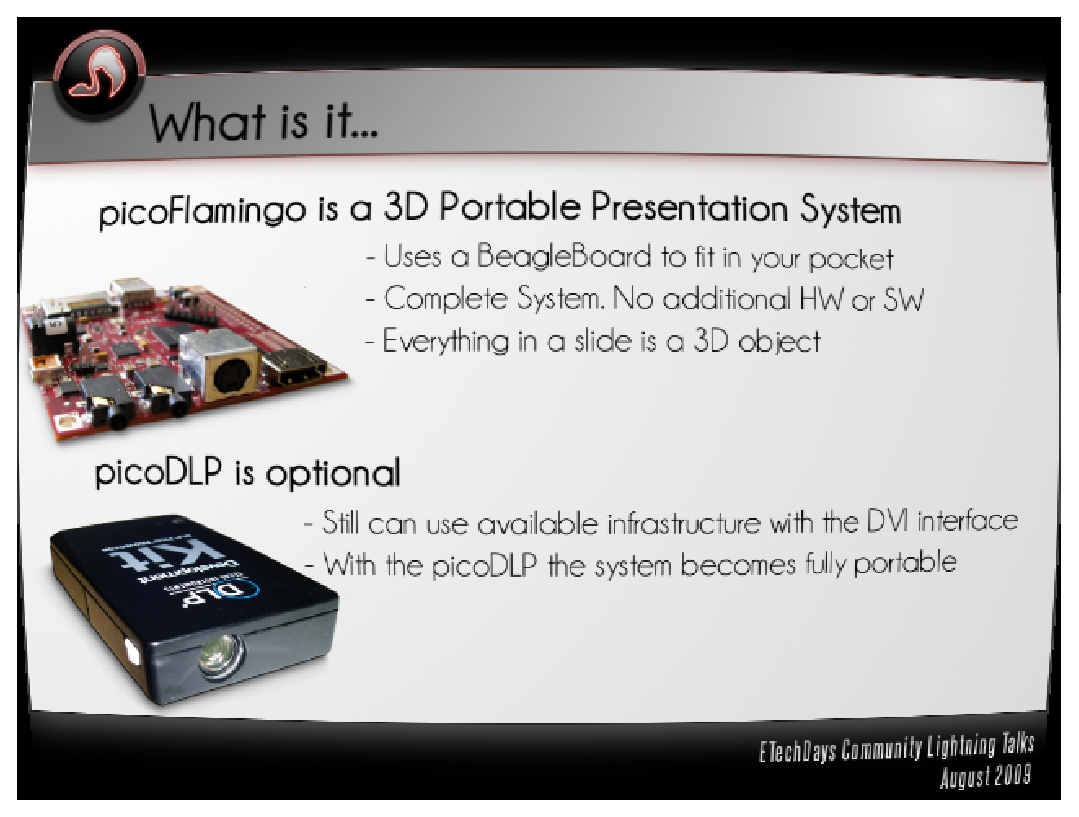
\includegraphics[width=0.7\hsize,angle=0]{images/post-proc2.eps}
{\small{\caption{\label{fig:post-proc2}The ``Cracking Egg'' post
      processing shader. Distortion correction}}}
\end{figure}




\subsection{Adding Text Styles}

The ``Cracking Egg'' provides a very simplistic style management system to allow the users include their own fonts in their presentations.

Adding a new style to the presentation is a very simple process.

\begin{itemize}
\item Add your True-Type font file (.ttf) into the fonts directory. 
\item Update the \verb!font_list.txt! file. This file is in the same directory that the ``Cracking Egg'' main application. The format for this file is as follows:

\verb!FontPointSize StyleName TruTypeFile!

where:

\begin{itemize}
\item \verb!FontPointSize! is the size in points of the font. The
  bigger this number the better the quality of the text in the
  presentation, but also, the most memory used. A value of 32 is
  normally enough to achieve an affordable quality. 

\item \verb!StyleName! is the user name for this style. This name will
  be used in the slides to select the text style for the text items. 

\item \verb!TrueTypeFile! is the name of the ttf file in the fonts
  directory to use for this style.

\end{itemize}
\end{itemize}


\clearpage
\pagebreak

\section{Running the Remote Control Applications}

This section explains how to run the different remote control
solutions for picoFlamingo ``Cracking Egg''.

\subsection{Command Line Control}

The picoFlamingo ``Cracking Egg'' can be controlled from the command line
using the commands described in section \ref{sec:control}. These
commands can be issued in the following ways.

\begin{itemize}
\item Using a communication tool like Netkitty or Netcat and
  connecting to one of the external interfaces provided by the
  system. These interfaces can be a TCP (wired or wifi) connection or
  a bluetooth RFComm connection (this only using NetKitty).
\item Directly typing in the console where the application was
  launched if available.
\end{itemize}

\subsection{Simple Remote Control for Python S60}

This application connects directly to the Bluetooth address hard coded
in the script. It read the device cursor keys. The right cursor key
sends a next slide command, and the left cursor key sends a previous
slide command.

\subsection{Extended Remote Control Application}

This application can be executed in different platforms once installed
as explained in \ref{sec:extended-control-app}. This application needs
a communication tool to remotely connect to the picoFlamingo ``Cracking
Egg'' system.

To achieve this goal, the application should be launched using a
command similar to the ones below:

\bigskip

\textbf{Connection using TCP networking}

\verb!pf-control | nk -client T:pink_egg_ip:port!

\bigskip

\textbf{Connection using BlueTooth}

\verb!pf-control | nk -client B:pink_egg_bt_addr:channel!


The specific TCP port or Bluetooth channel will depend on the way the
picoFlamingo ``Cracking Egg'' is started.

Once started the application will show an screen like the one on the
left of Figure \ref{fig:control-screen}.

\begin{figure}[ht]
\centering
  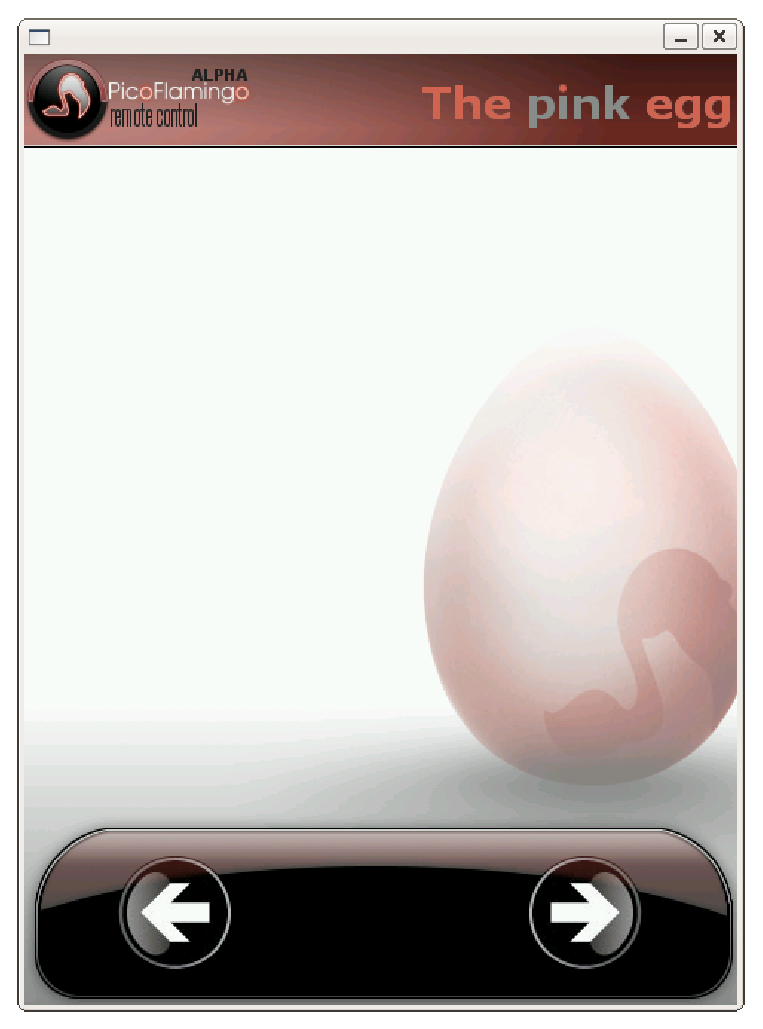
\includegraphics[width=0.45\hsize,angle=0]{images/pf-control.eps}  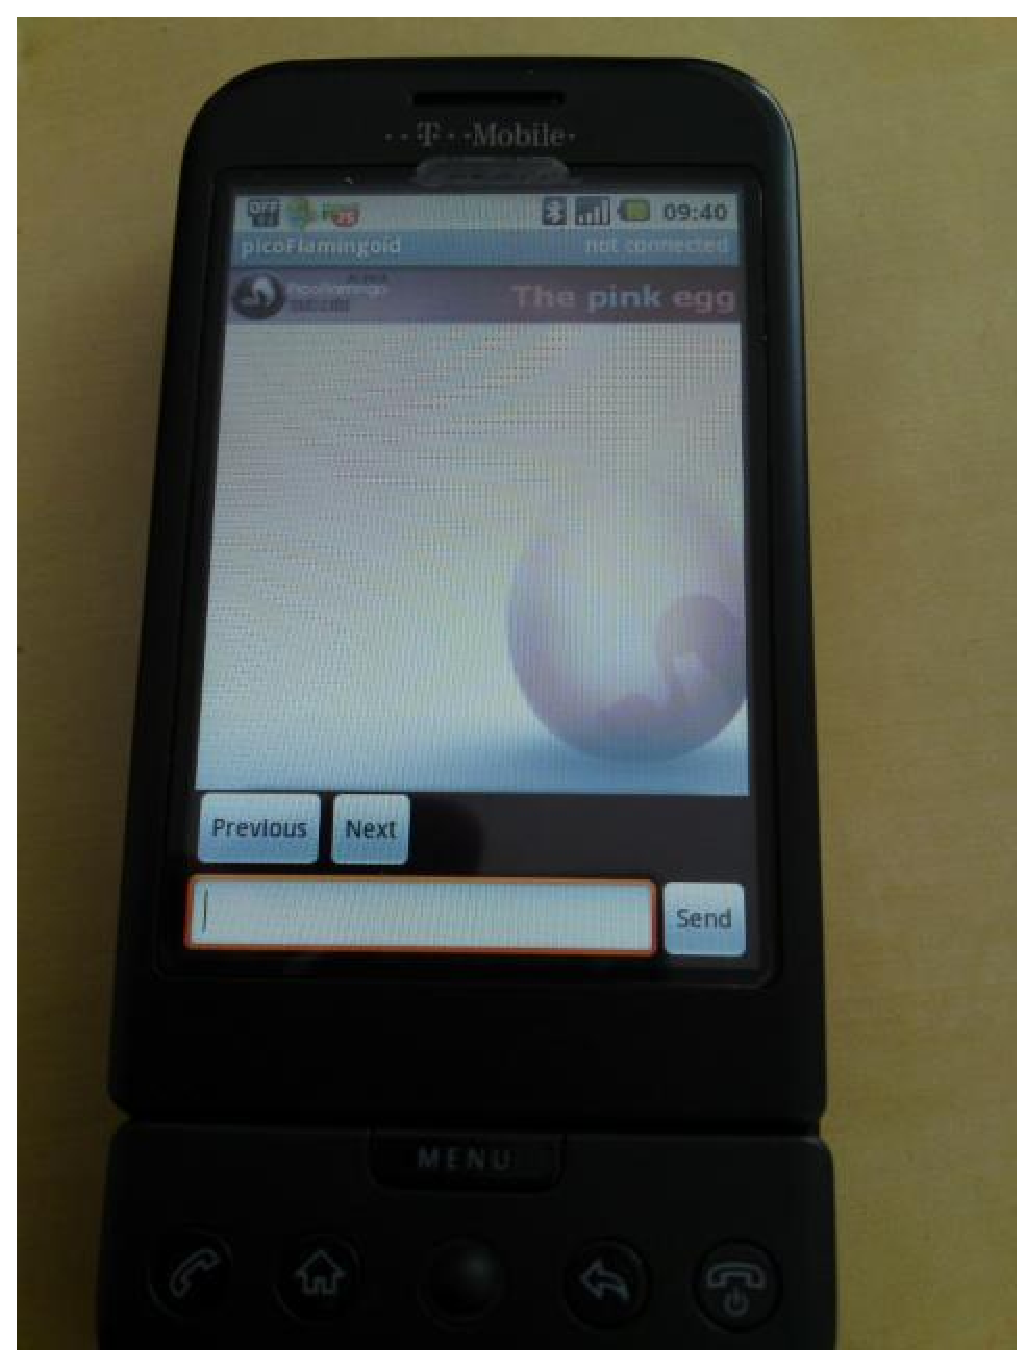
\includegraphics[width=0.45\hsize,angle=0]{images/picoflamingoid.eps}
\caption{\label{fig:control-screen}Extended Remote Control Application
(left) and early Android prototype -picoFlamingoid- (right)}
\end{figure}

The screen is divided in three main zones.

\begin{itemize}
\item The upper part of the screen shows some descriptive information
  about the tool. Clicking or touching is part of the screen will
  close it.
\item The lower part of the screen provides two navigations buttons to
  move forward and backwards through the presentation.
\item Finally, the central part of the screen is used to interact with
  the slide item having the focus. Pressing in this area will send a
  rotation command to the picoFlamingo ``Cracking Egg'' and the current
  focused item will be rotated accordingly.

  The interface only sends X and Y rotation angles. This angles are
  calculated proportionally to the distance in the X and Y axis
  between the center of the screen and the point the user clicked or
  touched the screen.
\end{itemize}

This interface is being extended to support several new features that
are being added and will change in future, including more different
operational models.

This interface has been successfully tested with the picoFlamingo
``Cracking Egg'' from an x86 PC and from a Free Runner OpenMoko phone. 

There is also a preliminary version of an Android application for
remote controlling picoFlamingo. The prototype is shown on the right
side of Figure \ref{fig:control-screen}. This application can also be
downloaded from the picoFlamingo website, but it is not included in
the source code distribution.



\clearpage
\pagebreak

\section{Video Streamer Applications}
\label{sec:video-streamer}

picoFlamingo the ``Cracking Egg'' includes a simple video streamer
application to feed real-time live video (from a webcam for instance)
into a picoFlamingo image item in a slide.

This video streamer uses libjpeg to compress the captured images and
works with v4l2 devices.

\subsection{Installation}

picoFlamingo video streamer is distributed as source code. In order to
compile the application the v4l2 headers are needed and the
development package of libjpeg needs to be installed in the system.

Once these requirements are fulfilled simply move to
\verb!app/video_server! and execute \verb!make!. Then the produced
executable needs to be copied to some directory included in the system
\verb!PATH! variable.

\subsection{Command line arguments}

The video streamer application distributed with ``The Cracking Egg''
accepts the following command line arguments:

\begin{itemize}
\item \verb!--device name! specifies the v4l2 device to be use for
  acquiring images. Default value is \verb!/dev/video0!
\item \verb!--width w! specifies the width of the images to be captured
\item \verb!--height h! specifies the height of the images to be captured
\item \verb!--port p! specifies the TCP port the server will accept
  connections to transmit the captured images
\item \verb!--format n! specifies the image format delivered by the
  v4l2 device. A value of 0 means that the images are delivered as
  compressed JPEG streams. A value of 1 means that the images are
  delviered as YUYV. The video streamer application will convert, in
  any case, the acquired images from the v4l2 devices into a JPEG
  coded image.
\end{itemize}

\subsection{Usage}

Please refer to section \ref{cmd-img} for details on how to feed
images from the video streamer into a picoFlamingo ``The Cracking
Egg'' image item.

\subsection{Hardware Supported}

The video streamer application distributed with picoFlamingo ``The
Cracking Egg'' should work with any v4l2 compliant device. The
following devices have been successfully used with the application:

\begin{itemize}
\item Logitech Webcam Pro 9000 (uvc driver) (YUYV format)
\item OMAP Zoom II built-in camera (YUYV format)
\end{itemize}

\clearpage
\pagebreak

\section{Voice Commanding Applications}

picoFlamingo ``The Cracking Egg'' includes a voice commanding
application based on Julius voice recogniser. This application allows
to navigate a presentation using the voice commands \verb!NEXT! and
\verb!PREVIOUS!.

\subsection{Installation}

picoFlamingo voice commanding application is distributed as source
code. In order to compile the application the Julius speech recogniser
and as suitable sound device for the target platform needs to be
already configured.

Once these requirements are fulfilled simply move to app/speech
directory and execute \verb!make!. Then the produced executable needs
to be copied to some directory included in the system \verb!PATH!
environmental variable

\subsection{Extra data files}

The voice commanding tool included with picoFlamingo needs an acoustic
model and grammar to effectively recognise the speaker voice. These
files can be obtained from the quick start package distributed by
voxforge.org:

\url{http://www.voxforge.org/home/downloads#QuickStart%20Anchor}

Then follow the instructions below:

\begin{itemize}
\item Download the quickstart package and uncompress in your system.
\item Copy the grammar file distributed with picoFlamingo into the
  \verb!grammar! directory
\item Run the command \verb!./bin/mkdfa.pl grammar/sample!. This will
  process the picoFlamingo grammar and produce the files required by
  Julius to interpret the navigation commands
\end{itemize}

In order to execute the application run the following command in the
quick start package directory:

\begin{verbatim}
$ ./julius-simple -input mic -C julian.jconf
\end{verbatim}

\subsection{Usage}

The voice commanding tool relies on the NetKitty application to
connect to picoFlamingo. The usual way to execute the tools is with
the following command line:

\verb!$ ./julius-simple -input mic -C julian.jconf | nk -client localhost 5000!

This command starts the voice commanding application using the local
microphone and the grammar produced in the previous section, and
forwards the recognised commands to post 5000 in the local
machine. 

Then picoFlamingo should be launch together with NetKitty listening in
port 5000.

For instructions on how to setup this tool to get the audio from a
different machine, please check this site:

\url{http://papermint-designs.com/community/?q=node/61}

For Julius/audio related troubleshooting please refer to the appropriated forums.

\clearpage
\pagebreak

\section{Creating Presentations}

In this release, a presentation is a sequence of slides. Each slide is
stored in a separated file named as `\verb!slideN.pfs!, where N is the
slide number. In order to create a presentation, the user has to create
a subdirectory and put on it one of these slideN.pfs files for each slide
s/he wants to show.

As explained above, the \verb!--reload! command line flag is very
useful when creating a presentation as it will show the changes made
in the slide file as they are made. 

{\textbf{NOTE. The --reload flag is broken on current release}}

Therefore, in order to create a presentation the format of the slides
(the .pfs file formats) needs to be known. 

The rest of this section describes this file format.

\subsection{Comments}
The .pfs file formats considers a comment any line starting with the
character ';'. Note that this character HAS TO be in the first column
of the line to comment out (no other character before it). 

\textbf{Example}

\begin{verbatim}
; This is a .pfs comment.
\end{verbatim}

\subsection{Slide Items}

This section describes the main items that can be added to a slide.

\subsubsection{BACKGROUND}

The command \verb!BACKGROUND! sets up the presentation background. The
background has to be an image in one of the supported formats. Slide
transition effects does not apply to the item index 0. In general the
\verb!BACKGROUND! command should be the first one in order to not be
affected by slide transitions.


\bigskip

\textbf{Syntax}

\verb!BACKGROUND image_file!

where

\begin{itemize}
\item \verb!image_file!, image file to add as a presentation background.
\end{itemize}

The background item has the additional property of not being affected
for the transition effects.

\bigskip

\textbf{Example}
\begin{verbatim}
; Background
BACKGROUND background3.png
\end{verbatim}

\subsubsection{ADD\_TEXT and ADD\_STEXT}

The \verb!ADD_TEXT! command adds a dynamic text item to the current
slide. The \verb!ADD_STEXT! command adds a static text item to the
current.

A static text item can be rendered faster but it cannot be updated
once initialised. Dynamic text items can be updates at any time,
changing any of their properties, including their content.

\bigskip

\textbf{Syntax}

\verb!ADD_TEXT text_style!

where

\begin{itemize}
\item \verb!text_style! is one of the valid text styles defined in the
  \verb!font_list.lst! file for the current presentation.
\end{itemize}

To change general properties for this item check the section
{\ref{sec:properties}}.

The \verb!ADD_TEXT! command supports the following subcommands to add
extra information to the item:

\begin{itemize}
\item \verb!ADD_DATA!. This subcommand adds a new text line to a text
  item.
\item \verb!SET_TEXT_INTERLNE!. This subcommand modifies the inter
  line separation for the current text item.
\item \verb!SCALE!. This subcommand modifies the size of the current
  text item. The expected value is the divisor for the text sizes.
\end{itemize}

\bigskip

\textbf{Example}
\begin{verbatim}
ADD_TEXT text01
; Text Data
SET_TEXT_INTERLINE 0.6
SCALE 100.0
ADD_DATA SLIDESHOW:
ADD_DATA EDIT SLIDE 5:
; General Item Properties
POSITION -3.0 1.2 -3.5
COLOR 0.9 0.9 0.9 0.9
\end{verbatim}

\subsection{ADD\_IMAGE and ADD\_CENTERED\_IMAGE}

The \verb!ADD_IMAGE! and \verb!ADD_CENTERED_IMAGE! commands adds an image to the current slide. 

\bigskip

\textbf{Syntax}

\verb!ADD_IMAGE scale imagefile!

where

\begin{itemize}
\item \verb!scale! is the size of the image and
\item \verb!imagefile! is the image file to add.
\end{itemize}

The \verb!ADD_IMAGE! maps the given image as a texture into a QUAD
running from coordinates (0,0) to (1,1). The \verb!ADD_CENTERED_IMAGE!
commands does the same but using a QUAD from (-0.5, -0.5) to (0.5, 0.5).

To change general properties for this item check the section
{\ref{sec:properties}}.

\bigskip

\textbf{Example}
\begin{verbatim}
; Image
ADD_IMAGE 2.5 beagle.png
POSITION -2.8 -2.2 -3.0
\end{verbatim}


\subsection{ADD\_CUBE}

The \verb!ADD_CUBE! command adds a 3D cube model to the current
slide. 

\bigskip

\textbf{Syntax}

\verb!ADD_CUBE sizeX sizeY sizeZ!

where

\begin{itemize}
\item \verb!sizeX! is the cube size in the X axis.
\item \verb!sizeY! is the cube size in the Y axis.
\item \verb!sizeZ! is the cube size in the Z axis.
\end{itemize}


To change general properties for this item check the section
{\ref{sec:properties}}. {\em Note: The color property cannot be
  changed for 3D Models in this version}

\bigskip

\textbf{Example}
\begin{verbatim}
;Interactive Cube
ADD_CUBE 1.5 1.0 1.0
SET_FOCUS
POSITION -0.0 -0.2 -3.0
ROTATION 0.7 0.2 0.0
\end{verbatim}



\subsection{ADD\_MODEL}

The \verb!ADD_MODEL! command adds a 3D model to the current
slide. 

\bigskip

\textbf{Syntax}

\verb!ADD_CUBE model_file!

where

\begin{itemize}
\item \verb!model_file! is the file name of a 3D model on 3DS format
\end{itemize}


To change general properties for this item check the section
{\ref{sec:properties}}. {\em Note: The color property cannot be
  changed for 3D Models in this version}

\bigskip

\textbf{Example}
\begin{verbatim}
;Interactive Cube
ADD_MODEL 3D1.3d
SET_FOCUS
POSITION 0.0 0.2 -3.0
\end{verbatim}



\subsection{General Item Properties}
\label{sec:properties}
This section describes the commands used to set general item properties.

\subsection{NAME}

The \verb!NAME! command allows to provide a symbolic name to the item
currently being defined. This name can be used to give the item the
focus or to reference it with the FX commands

\bigskip
\textbf{Syntax}

\verb!NAME name!

where

\begin{itemize}
\item \verb!name! is a string.
\end{itemize}


\bigskip
\textbf{Example}

\begin{verbatim}
ADD_CUBE 1.5 1.0 1.0
NAME my_cube
\end{verbatim}




\subsubsection{POSITION}

The \verb!POSITION! command allows the user to set the position in the
slide for the current item.

\bigskip
\textbf{Syntax}

\verb!POSITION X Y Z!

where

\begin{itemize}
\item \verb!X Y Z! are the 3D position for the current item.
\end{itemize}


\bigskip
\textbf{Example}

\begin{verbatim}
ADD_CUBE 1.5 1.0 1.0
POSITION -0.0 -0.2 -3.0
\end{verbatim}


\subsubsection{ROTATION}

The \verb!ROTATION! command allows the user to set the rotation in the
slide for the current item.

\bigskip
\textbf{Syntax}

\verb!ROTATION A B C!

where

\begin{itemize}
\item \verb!A B C! are the 3D rotation w.r.t. the X, Y, Z axis  for
  the current item. Angles are in radians.
\end{itemize}


\bigskip
\textbf{Example}

\begin{verbatim}
ADD_CUBE 1.5 1.0 1.0
POSITION -0.0 -0.2 -3.0
ROTATION 0.7 0.2 0.0
\end{verbatim}



\subsubsection{COLOR}
The \verb!COLOR! command allows the user to change the color of a
given item. {\em Note: this command doesn't work on 3D models in this release}.

\bigskip
\textbf{Syntax}

\verb!COLOR R G B ALPHA!

where:

\begin{itemize}
\item \verb!R G B, ALPHA! is a 4D vector specifying the color to
  apply, including the alpha channel. 
\end{itemize}

\bigskip
\textbf{Example}

\begin{verbatim}
ADD_TEXT text07
ADD_DATA ... much more coming soon!!!
POSITION -2.0 -2.6 -3.5
SCALE 100.0
COLOR 0.1 0.1 0.1 0.8
\end{verbatim}

\subsection{Other Commands}
This section introduce other commands not directly related to the
slide items.

\subsubsection{INCLUDE}
The \verb!INCLUDE! command allows the inclusion of an external file
containing picoFlamingo ``Pink Egg'' commands in the current slide.

\bigskip
\textbf{Syntax}

\verb!INCLUDE template_file!

where:

\begin{itemize}
\item \verb!template_file! is the file to include in the current slide.
\end{itemize}

\bigskip
\textbf{Example}

\begin{verbatim}
; Include common header for presentation
INCLUDE header.pfi
\end{verbatim}

\subsubsection{SET\_FOCUS}
The \verb!SET_FOCUS! command, indicates
to the system that the given item has the focus and will receive any
interactive command from the remote system interfaces.

The \verb!SET_FOCUS! command can only be applied after the slide is
defined (dynamically at run-time) or between a \verb!FX_START!,
\verb!FX_END! block within the slide

\bigskip
\textbf{Syntax}

\verb!SET_FOCUS my_cube!

\bigskip
\textbf{Example}

\begin{verbatim}
; Remote Controlled Spining Cube
ADD_CUBE 1.5 1.0 1.0
NAME my_cube
POSITION -0.0 -0.2 -3.0
ROTATION 0.7 0.2 0.0
FX_START
SET_FOCUS my_cube
FX_END
\end{verbatim}


\subsubsection{GENERIC\_EVENTS}

The \verb!GENERIC_EVENTS! command indicates to picoFlamingo if the
mouse vents received on X11 mode should be interpreted as commands for
the current item with the focus or should be forwarded to other
application using \verb!stdout!.

\bigskip
\textbf{Syntax}

\verb!GENERIC_EVENTS n!

where:

\begin{itemize}
\item \verb!n! can be 0 (events manipulate current slide item) or 1
  (events are forwarded to stdout)
\end{itemize}




\subsubsection{SHOW}

The \verb!SHOW! command indicates to the system if a given slide item
has to be shown or hidden.

\bigskip
\textbf{Syntax}

\verb!SHOW name n!

where:

\begin{itemize}
\item \verb!name! represents the name of the item to show or hide
\item \verb!n! can be 0 (item is hidden) or 1 (item is shown)
\end{itemize}


\bigskip
\textbf{Example}

\begin{verbatim}
; Remote Controlled Spining Cube
ADD_CUBE 1.5 1.0 1.0
NAME my_cube
POSITION -0.0 -0.2 -3.0
ROTATION 0.7 0.2 0.0
FX_START
SHOW my_cube 0
FX_END
\end{verbatim}


\subsection{Text Manipulation Commands}

The following commands can be used to manipulate the dynamic text
(text items created with command \verb!ADD_TEXT!) rendering.

\begin{itemize}
\item \verb!SET_TEXT_INTERLINE name interline! . 

Changes the interline
  space between the lines of the \verb!name! slide text item


\item \verb!UPDATE_TEXT_INTERLINE name interline!. 

Dynamically changes
  the interline space between the lines of the \verb!name! slide text item.


\item \verb!UPDATE_FONT name font_name!. 

Dynamically updates the
  associated font to the \verb!name! slide text item.


\item \verb!UPDATE_TEXT_SCALE name scale_x scale_y!. 

Dynamically
  changes the X and Y scale for the slide text item \verb!name!


\item \verb!UPDATE_TEXT_WIDTH name width!. 

Dynamically updates the
  fixed width associated to \verb!name! text item in the slide


\item \verb!UPDATE_TEXT name new_text!. 

Dynamically changes the
  content of \verb!name! text item.


\item \verb!TXT_SET_LINE name num_line!. 

Sets the initial line for a
  multi-line text item.


\item \verb!TXT_SET_LINES_UP name lines_up!. 

Indicates how many lines
  up of the current line will be rendered.


\item \verb!TXT_SET_LINES_DOWN name lines_down!. 

Indicates how many
  lines down of the current line will be rendered.


\end{itemize}

\subsection{Image Manipulation}
\label{cmd-img}
The following command can be used to manipulate images

\begin{itemize}
\item \verb!SET_IMAGE name file_name!. Allows to load a new image file
  into the image slide item \verb!name!. {\textbf{Current version
      requires the new image to be the same width and height that the
      current one}}
\item \verb!CONNECT name ip port!. Connect to a video streamer server
  (Section \ref{sec:video-streamer}) and starts rendering the video stream in
  the image item \verb!name!.  {\textbf{Current version requires the
      video stream an the target image to have the same width and height}}
\item \verb!DISCONNECT name!. Disconnect image \verb!name! from any
  video streamer associated to it.
\item \verb!SHOT_WIDTH_NAME name file_name!. Saves current video stream frame
  associated to image \verb!name! into a JPEG file with the provided name.
\end{itemize}

\subsection{Special Effects and Animation}

The following command can be used to animate slide items

\begin{itemize}
\item \verb!FX_START!. 

Starts the FX definition section in a slide   file. 
\item \verb!FX_END!. 

Indicates that the FX section in the slide file ends


\item \verb!FX_POS name frame_0 duration X0 Y0 Z0 X1 Y1 Z1!. 

Initiates
  a position animation on item \verb!name!, starting at frame
  \verb!frame_0! relative to the time the comment was issued, for
  \verb!duration! frames, moving the item from position
  \verb!(X0,Y0,Z0)! to position \verb!(X1,Y1,Z1)!


\item \verb!FX_MOVE_TO name frame_0 duration X1 Y1 Z1!. 

Initiates
  a position animation on item \verb!name!, starting at frame
  \verb!frame_0! relative to the time the comment was issued, for
  \verb!duration! frames, moving the item from its current position
  to position \verb!(X1,Y1,Z1)!



\item \verb!FX_ROT name frame_0 duration H0 P0 R0 H1 P1 R1!. 

Initiates
  a rotation animation on item \verb!name!, starting at frame
  \verb!frame_0! relative to the time the comment was issued, for
  \verb!duration! frames, rotating the item from angles
  \verb!(H0,P0,R0)! to angles \verb!(H1,P1,R1)!

\item \verb!FX_ROT_TO name frame_0 duration H1 P1 R1!. 

Initiates
  a rotation animation on item \verb!name!, starting at frame
  \verb!frame_0! relative to the time the comment was issued, for
  \verb!duration! frames, rotating the item from its current orientation
  to orientation \verb!(H1,P1,R1)!


\item \verb!FX_COLOR name frame_0 duration R0 G0 B0 A0 R1 G1 B1 A1!. Initiates
  a color animation on item \verb!name!, starting at frame
  \verb!frame_0! relative to the time the comment was issued, for
  \verb!duration! frames, changing item from color
  \verb!(R0,G0,B0, A0)! to color \verb!(R1,G1,B1, A1)!

\item \verb!FX_COLOR_TO name frame_0 duration R1 G1 B1 A1!. 

Initiates
  a color animation on item \verb!name!, starting at frame
  \verb!frame_0! relative to the time the comment was issued, for
  \verb!duration! frames, changing the item from its current color
  to color \verb!(H1,P1,R1)!

\end{itemize}

In addition to the frame based animation commands described above, a
time-based version of all those commands is also available. For these
time based version, the parameters \verb!frame_0! and \verb!duration!
should be identified as initial time (in milliseconds) and duration
(also in milliseconds

The time based animation commands are, respectively:
\verb!FX_TPOS!, \verb!FX_TROT!, \verb!FX_TCOLOR!, \verb!FX_TMOVE_TO!,
\verb!FX_TROT_TO! and \verb!FX_TCOLOR_TO!.



\subsection{Controlling the Presentation}
\label{sec:control}
The ``Cracking Egg'' release only supports three control commands. This commands can be issued directly from the console (if netkitty is not used), or remotely through bluetooth or TCP/IP networking (using netkitty or netcat).

The available commands are:

\begin{itemize}
\item \textbf{NEXT}: Goes to next slide in presentation.
\item \textbf{PREV}: Goes to previous slide in presentation.
\item \textbf{SLIDESHOW}: Switches ON/OFF slideshow mode.
\item \textbf{ROT X Y Z}: Rotates the current presentation item
  with respect to the three main axis.
\end{itemize}





\clearpage
\pagebreak


\section{Known Issues}

This is a very early alpha version that is very buggy and it is only
intended to give future users a feeling of what picoFlamingo can
offer. This version is simply a quick integration of the different
tests carried out so far and, therefore should be considered as a
macro test. 

In any case, there are some already know issues with this version.

\begin{itemize}
\item There is no proper error management. If something is wrong (a
  very big image, a wrong scale value or an improper SGX
  configuration) the application will simply crash. 

\item The specific configuration for U-Boot and Linux kernel seems to
  be a bit tricky and we were only able to make it work with the
  configuration stated above. 

\item The \verb!ROTATION! command has some issues with image
  transparency and doesn't rotates properly text items.

\item The texture manager object has not yet been added so a texture
  is created for each single image used (even when used several
  times), so images should be used carefully.

\item U-Boot 2009.1-dirty is required for USB Host operation on
  BeagleBoard C3.  This version seems to no longer take the
  environment from NAND so a simple \verb!saveenv! do not work, when
  using U-Boot from the SD card.

  In order to pass the proper command line to the kernel to initialise
  the graphics in 16bpp mode, the U-Boot booting process can be
  interrupted from the console, the proper variable set and the
  \verb!boot! command used for one-time booting. This has to be done
  each time the system is rebooted.

  The easiest way to avoid this is to Flash U-Boot to NAND so the
  \verb!saveenv! command will work properly. Otherwise a proper U-Boot
  script needs to be provided

\end{itemize}



\clearpage
\pagebreak
%\printindex

\pagestyle{empty}
\rput(8,-11.5){\resizebox{21cm}{32cm}{{\epsfbox{images/back-page.eps}}}}
\end{document}
